\chapter{Implementation}

According to \cite{wolf}, the most effective language for the implementation of LGCA is C, with slightly better performance than Fortran.
In our implementation, we could not resist to use some comfortable features of C++, but we have sticked to the low-level C-style of programming.
\bigskip

%We listened to this advice and started the implementation in C language, but we could not resist to use some "shortcuts" of C++, but we stayed true to the C-style of programming.
%
%\bigskip

%The programs have substantially grew over the time, and in case of further development,

%and we got on the crossroad how to efficiently develop our two models further. The current option number one (in the process while writing these lines) is to use the pure C, and pack it as \textit{extension module} to Python, mainly for our own comfort in future applications, but we would be glad if it finds its way to some fellow out there.

\section{Parallelization}
Languages C and C++ offer three widely used interfaces for parallelization:
\begin{enumerate}
\item OpenMP
\item MPI
\item Cuda
\end{enumerate}
%
%We rather obey the old Chinese saying 
%\begin{CJK*}{UTF8}{gbsn}
%'谁闻起来像腋下汗湿的龙,不应该使用 Cuda', so Cuda is obviously out of the question.
%\end{CJK*}

\bigskip

MPI was our hot candidate from the beginning and we have even used it on the $1D$ cellular automaton with range 2. 
%But after consulting the experienced colleague, we concluded that OpenMP would be more appropriate choice.
But in the end, we concluded that OpenMP would be more appropriate choice.
Since we have opporunity to use clusters at Metacenter (the network of academic clusters in the Czech republic) we expected we could employ huge amount of processors, if we use MPI and compute on various clusters parallely. But we learnt that in the practice we can hardly employ more then two hundreds of processors.
Using OpenMP, we can run the computation on SMP machine with 64 processors, which is not significantly lower.

The drawbacks of MPI are obvious, it requires vast modification of the code, contrary to OpenMP that usually requires only several lines of code to add.

Moreover, parallelization with OpenMP can be easily included to Python extension module.

In the following section, we provide a useful measure of our parallel implementation, the \textit{scaling efficiency}. It indicates the speedup of the computation with the increasing number of processing units employed.
We applied two distinct concepts of scaling efficiency.

\section{Strong scaling}
In strong scaling measurement, we vary the number of processing units, while the problem size stays fixed.

The formula is as simple as
\begin{align*}
s_N = \frac{t_1}{N t_N} 100\%,
\end{align*}
where $t_1$ is a time to finish the work with one processing unit and $t_N$ is time to finish the same amount of work with $N$ processing units.

The idea of strong scaling is to find a "sweet spot" -- optimal number of computational units to compensate for the overhead of parrallelisation.
%relative to the overhead ...
\section{Weak scaling}
In this measurement, we vary number of processing units, but we vary also the size of the problem accordingly, so that amount of work per one processing unit is constant.

The weak scaling formula reads
\begin{align*}
w_N = \frac{t_1}{t_N} 100\%,
\end{align*}
where $t_1$ is time to complete $1$ unit of workload with $1$ processing unit, while $t_N$ is time to complete $N$ units of workload with $N$ processing units.

Therefore, the weak scaling tells us how requirements on memory bandwidth and other resources depend on the size of the problem.

\section{Flow on the sphere}
The most time--consuming simulation that we performed was the turbulent flow inside the sphere simulated by Pair-interaction, so the measurement of scaling on this problem is of the highest importance.

The strong scaling was measured on the sphere with diameter $d = 500$ over $3000$ time-steps.
On the graph below, we plotted time--length of the last $1000$ steps against the number of cores employed.
\begin{figure}[H]
 \centering 
 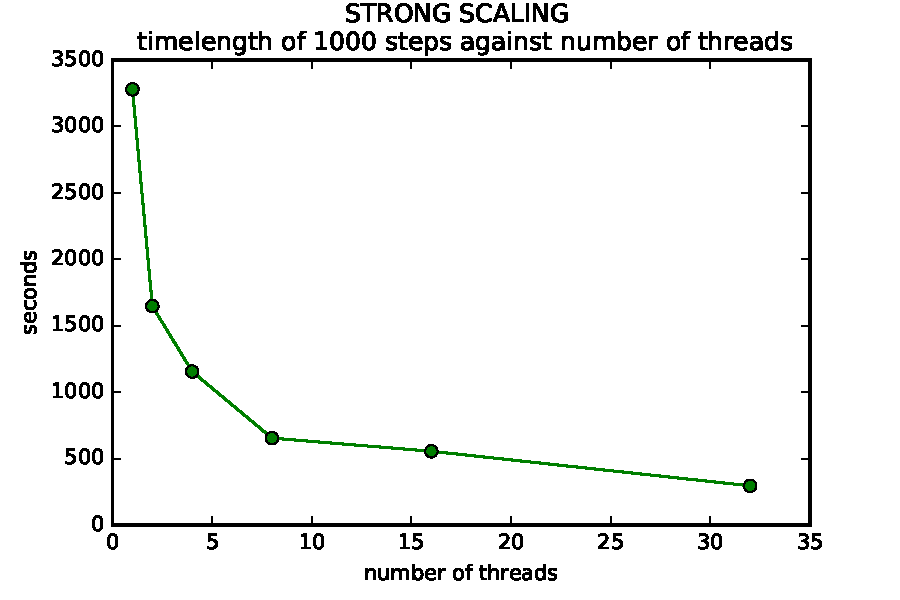
\includegraphics[width=1\textwidth]{./img/strongscalingg}
\end{figure}

For the weak scaling, the diameter of the sphere varied, so that the volume of lattice was increasing proportionally to the number of threads. However, side of the lattice must be multiple of $10$, because macroscopic velocity is computed over the cube with side of $10$. Therefore, the number of nodes per one thread differs, but no more then by $5\%$.

\begin{tabular}{ |p{2cm}|p{4cm}|p{4cm}| }
 \hline
 Threads & Diameter [nodes] & Nodes per one thread \\
 \hline
 \hline
$1$ & $320$ & $32\,768\,000$ \\
 \hline
$2$ & $400$ & $32\,000\,000$\\
 \hline
$4$ & $500$ & $31\,250\,000$ \\
 \hline
$8$ & $630$ & $31\,255\,875$\\
 \hline
$16$ & $800$ & $32\,000\,000$ \\
 \hline
$32$ & $1000$ & $31\,250\,000$ \\
 \hline
 \end{tabular}


\begin{figure}[H]
 \centering 
 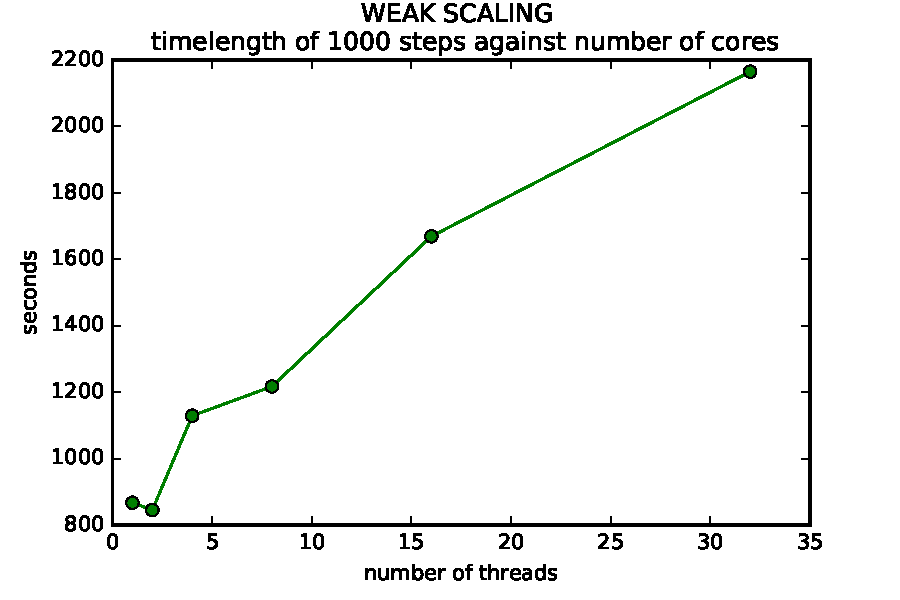
\includegraphics[width=1\textwidth]{./img/weakscaling}
\end{figure}

All computations were performed on the cluster \textbf{Alfrid} of \textit{University of West Bohemia}.

\begin{tabular}{ |p{4cm}|p{8.8cm}| }
\hline
\multicolumn{2}{|c|}{Alfrid cluster} \\
\hline
\hline
Architecture &          x$86\_64$ \\
\hline
CPU op-mode(s) &        32-bit, 64-bit \\
\hline
Byte Order &            Little Endian \\
\hline
CPU(s) &                32 \\
\hline
On-line CPU(s) list &   0-31 \\
\hline
Thread(s) per core &    2 \\
\hline
Core(s) per socket &    8 \\
\hline
Socket(s) &             2 \\
\hline
NUMA node(s) &          2 \\
\hline
Vendor ID &             GenuineIntel \\
\hline
CPU family &            6 \\
\hline
Model &                 62 \\
\hline
Model name &            Intel(R) Xeon(R) CPU E5-2650 v2 @ 2.60GHz \\
\hline
Stepping &              4 \\
\hline
CPU MHz &               1216.007 \\
\hline
CPU max MHz &           3400.0000 \\
\hline
CPU min MHz &           1200.0000 \\
\hline
BogoMIPS &              5201.43 \\
\hline
Virtualization &        VT-x \\
\hline
L1d cache &            32K \\
\hline
L1i cache &            32K \\
\hline
L2 cache &            256K \\
\hline
L3 cache &              20480K \\
\hline
NUMA node0 CPU(s) &     0-7,16-23 \\
\hline
NUMA node1 CPU(s) &     8-15,24-31 \\
 \hline
 \end{tabular}

%In the following chapter, we offer brief discussion of the most important parts of our source code.